\documentclass[a4paper]{article}

\usepackage[english]{babel}
\usepackage[utf8x]{inputenc}
\usepackage{amsmath}
\usepackage{graphicx}
\usepackage[colorinlistoftodos]{todonotes}

\usepackage{authblk}

\bibliographystyle{ieeetr}

\title{Personalized Recommendation System for Questions to Answer on SuperUser}
\author{Group 44: Geza Kovacs, Arpad Kovacs, Shahriyar Pruisken}
\date{December 10, 2013}

\begin{document}


\maketitle

\begin{abstract}
We have built a personalized recommendation engine that is able to predict, at a given snapshot of time, the probability of a given user answering a particular SuperUser question. We use this in the application of generating personalized suggestions of questions that each user would be interested in answering.

We have developed 2 components to recommend relevant questions to users: one which computes the match in a question's topic to a potential answerer's interests, and another which predicts the likelihood of an answer coming in for a question at a given point in time. We combine these results by multiplying and normalizing to generate an overall estimate of the probability a question is answered by a given user at a given time.

We use community detection at the tag-similarity level to establish recommended questions for particular communities, and use this to diversity recommendations, particularly for users who have limited history on the site. Results show that our combined approach is more accurate at modeling question-answering events on a subset of the StackOverflow question-answering network than either of the individual components alone. Our final model is able to generate recommendations such that the actual question answered is among the 29 top recommendations .
\end{abstract}

%\begin{figure*}[ht]
%\centering
%
\includegraphics[width=\columnwidth]{example-user-tagcloud}
%\caption{Set of personalized recommendations generated for a user whose tag-cloud representing interests (tags of questions he has answered) is shown. As we can see, the top 10 recommendations include the question he ultimately ends up answering.}
%\label{fig:example-user-tagcloud}
%\end{figure*}

\section{Introduction}

Question-answering sites such as StackOverflow or SuperUser provide users with a wealth of questions that they can answer. However, some questions might be more relevant to the user than others - namely, they cover topics that users have indicated that they are interested in, by answering other questions in that topic. Other questions might be topically relevant, but aren't in need of answers due to temporal factors, and other factors associated with the overall question activity - specifically, the requester has indicated that they are already satisfied by a particular answer, or there have been so many answer submissions that there is nothing left to contribute, or the question might be so old that there it is no longer relevant.

Our objective in this paper is to develop a personalized recommendation system that identifies questions which a particular user might be interested in answering at a given point in time. We use users' actual history of answering questions as a proxy to model their actual history of answering questions - so under this model, if John answered a question about Excel at 2pm, then an optimal personalized recommendation system would have suggested that question to him if he had looked at his recommendation list at 1:59pm.

Our recommendation system generates recommendations by estimating how likely a particular question will be answered by the user at a particular time, and sorting questions according to this score to generate a list of recommendations. We develop 2 general classes of features to use for computing the probability that a user answers a given question at a particular time: \emph{topical-relevance} features dependent on the user, and \emph{question-activity} features dependent on the time and existing answering activity on the question.

Note that representating users' interests as the set of tags they have answered has a limitation, in that if a user has only answered very few questions, their set of tags will be heavily biased towards the questions they have answered, and will not cover all topics they might be interested in. For this reason, we use community detection to detect groups of users with common interests, match each user to a community, and weighted-average the user's tag set with their community's tag set. This provides benefits in predciting questions the user might be interested in, particularly for users with less history on the site.

We evalute our  recommendation system by running through the list of question-answering events that occur on SuperUser, and seeing what the rank of the question that was actually answered was in our recommendation system. We did our evaluation on SuperUser, a smaller sister site of StackOverflow, because we were having difficulty storing results in memory due to the sheer size of the StackOverflow dataset.
We have implemented the system which generates recommendation rankings, as well as the system which compares generated rankings to actual question-answering history to evaluate the system, but we were unable to run the full evaluation on the combined signal due to computational resource limitations. However we were able to individually evaluate both the topic-relevance as well as the question-activity models for the ranking tasks, and both show promising results.
%Our initial system, using a combined score, has a median rank of FILLME over these questions - so FILLME. This is an improvement over the individual scores of FILLME.

\section{Related Work}

Content-based recommendation systems analyze the content that the user tends to interact with, in order to generate recomendations \cite{pazzani2007}. For typical contexts such as suggesting relevant pages to read, finding a match between the content and the user's interests is the primary goal \cite{ansari2000}. These systems use statistical methods to find the essential parts of the content that are relevant to making recommendations to users - for example, using TF-IDF, which is the ratio of term frequency relative to the overall frequency in the domain, to find important keywords and tags that characterize the content \cite{pazzani2007}. This information is then captured in a weighted-vector representation, which we can then dot-product to create a linear-model \cite{lewis1996} for determining matches between user interests and content.

In the domain of recommendations on question-answering social networks such as SuperUser or StackOverflow, however, an additional dimension is introduced beyond just the question content itself - namely, the activity level on the question. Even if a question is completely relevant to the user's interests, if it has already been answered, or was asked several years ago, then they are considerably less likely to be interested in writing an answer for it. Anderson et al \cite{anderson2012} perform an analysis of StackOverflow, and develop a model for predicting which questions have been answered fully and will not be getting further answers. However, this work simply looks at features useful for predicting question activity patterns as a whole, and is not directly usable for generating personalized recommendations, because it works solely with the question metadata, and does not incorporate the content or user interests into its model.

The contribution we aim to make is to integrate both activity-level signals, as well as topic-relevance signals, to create a recommendation system for StackOverflow questions. By both considering factors such as activity level of a question, as well as personalizing question recommendations according to the match between question content and users, we can better model the questions a user will answer, than recommendations based on just one or the other class of features.

Our work is not the first recommendation system that incorporates temporal cues - Koren's NetFlix movie recommendation system incorporates temporal cues regarding movie freshness \cite{koren2010}. However, we believe the question-answering domain of StackOverflow is more rich than movie recommendations in external activities that affect user activity - such as other users answering questions - and hence we expect that temporal and activity cues will be even more useful and important for generating personalized StackOverflow question recommendations.

Herlocker et al provide an overview of ways to evaluate content recommendation systems \cite{herlocker2004}. There are 2 general approaches we can use: either generate recommendations and run user studies where we see whether they like the recommendations (as indicated by click-through rates and similar metrics), or offline experimenets where we attempt to predict user behavior simulated based on past data \cite{zaier2008}. As we are unable to actually run A/B tests and other user studies on StackOverflow, our evaluation uses the offline evaluation approach, predicting a particular user action - specifically, the answering of a question by a given user at a given point in time. Our evaluation also simulates the generation of recommendations for users at particular points in time - looking at what rank the question they end up answering is on the generated recommendation list.

Community detection allows us to find groups of related users in a graph \cite{fortunato2010community}. There has been much work in algorithms to quickly perform community detection \cite{communitybenchmarks}, of which we use the Louvian algorithm \cite{louvian}, which is relatively fast and considers edge weights between users in detecting communities.

\section{Features used for Generating Recommendations}

Our recommendation system generates recommendations by estimating how likely a particular question will be answered by the user at a particular time, and sorting questions according to this score.

Because we lack the computational resources to directly compute the probability of a question being answered by a given user at a given time, aka $P(Q|U,T)$, without making independence assumptions, then we use an independence assumption between users and time to instead allow us to compute a probability that a question will be answered by a given user, $P(Q|U)$, and the probability that a given question will be answered at a given time, $P(Q|T)$, and combine them.

Specifically, the math as is follows:

First, apply Bayes' rule:

\[ P(Q|U,T) = \frac{P(T,U|Q)P(Q)}{P(T,U)} \]

Apply conditional independence assumption $P(T,U|Q) = P(T|Q)P(U|Q)$

\[ P(Q|T,U) = \frac{P(T|Q)P(U|Q)P(Q)}{P(T,U)} \]

Substitute $P(U|Q)*P(Q) = P(U,Q)$

\[ P(Q|T,U) = \frac{P(T|Q)P(U,Q)}{P(T,U)} \]

Substitute $P(T|Q) = P(T,Q) / P(Q)$

\[ P(Q|T,U) = \frac{P(T,Q)P(U,Q)}{P(Q)P(T,U)} \]

Substitute $P(T,Q) = P(Q|T)*P(T)$

\[ P(Q|T,U) = \frac{P(Q|T)P(T)P(U,Q)}{P(Q)P(T,U)} \]

Substitute $P(U,Q) = P(Q|U)P(U)$

\[ P(Q|T,U) = \frac{P(Q|T)P(T)P(Q|U)P(U)}{P(Q)P(T,U)} \]

Using our independence assumptions, substitute $P(T,U) = P(T)*P(U)$

\[ P(Q|T,U) = \frac{P(Q|T)P(T)P(Q|U)P(U)}{P(Q)P(T)*P(U)} \]

Cancel $P(T)*P(U)$ in the numerator and denominator

\[ P(Q|T,U) = \frac{P(Q|T)P(Q|U)}{P(Q)} \]

We can compute the $P(Q)$ factor by summing over $P(Q,U)$ over all users.

So we have now broken down our problem into computing $P(Q|U)$, the probability a question will be answered by a given user, and $P(Q|T)$, the probability that a question will be answered at a given time. We develop 2 seperate models for computing these quantities: a \emph{topical-relevance} model for computing $P(Q|U)$, and a \emph{question-activity} model for computing $P(Q|T)$.

\section{Topical Relevance Model for Determining Relevance of a Question to a User's Interests}

In the context of StackOverflow, we can characterize question topics according to the tags that they have, and unigrams/bigrams that are present in the question title. We can characterize the topical interests of a particular user by considering the tags of questions they have previously answered. This allows us to compute a topical match score - the degree to which a particular question matches the user's interests, which indicates how interested a particular user might be in answering a question (independent of when the question was asked, or what answers have already been submitted).

In our current iteration, the topicality model is implemented by first developing a set of ``relevant tags'' for each user. We do this by first considering the set of tags for each of the questions a user has answered, and taking a union of all tags of questions they have answered thus far. Tags are weighted according to how many questions the user answers that the tag occurs in - so if a user answered 100 questions tagged ``OpenCV'' and only 1 question tagged ``Haskell'', then the OpenCV wll have a 100x larger weight for the user.

Then, for a new question associated with a set of tags, we can compute a topicality-relevance score to a user, by taking the user's set of tags, and dot-producting them against the set of tags in the new question. By taking an L2 norm (normalizing scores by the sum of squares) of each tag vector before dot-producting, this ensures that the resulting topical relevance score is between 0 and 1, with a score of 1 if the set of tags of the user and the question completely match, and a score of 0 if there is no overlap between the tags. Of course, we smooth our results using add-k smoothing to ensure that there will always be a small nonzero probability that a user will answer a question, even if there is no topical match.

We should note that not all tags are equally important. Specfically, a generic tag that is applied to a very wide range of questions - for example, ``programming'' - should have much less influence on the topicality match score, relative to a more specific and rare tag, such as ```SNAP.PY''. To account for this, we consider the probability of a tag not occurring in a randomly-chosen question, which is 1 - (\#questions in which tag appears)/(\#questions total), and we weigh the tags according to this. Note that the second quantity here is the TF-IDF, applied to tags \cite{pazzani2007}. This will ensure that additional weight is given to rarer, more specific tags.

%There are some questions on StackOverflow where the question is not tagged with enough tags, so our approach will work poorly for these. To address this issue, in our final version we aim to also extract out unigrams and bigrams from the title text of questions and lump these in with the tags, in case they contain information that the tags didn't contain, though we have not yet implemented this change.

We evaluated the Topicality Relevance model in isolation as follows. For each user, we computed the set of tags for the user, and ranked all questions according to their topicality-match scores for the user. These are essentially the questions which best match the user's tags, ignoring the question-activity and temporal components of the recommendation system. We then consider the set of questions which they did actually answer, and see what rank they have on this list. We did this for the top 10000 users, because we have sufficient amount of question-answering data for them that they have a relatively diverse set of tags. The resulting histogram of question ranks is displayed in \ref{fig:ranks-of-questions}.

\begin{figure*}[ht]
\centering
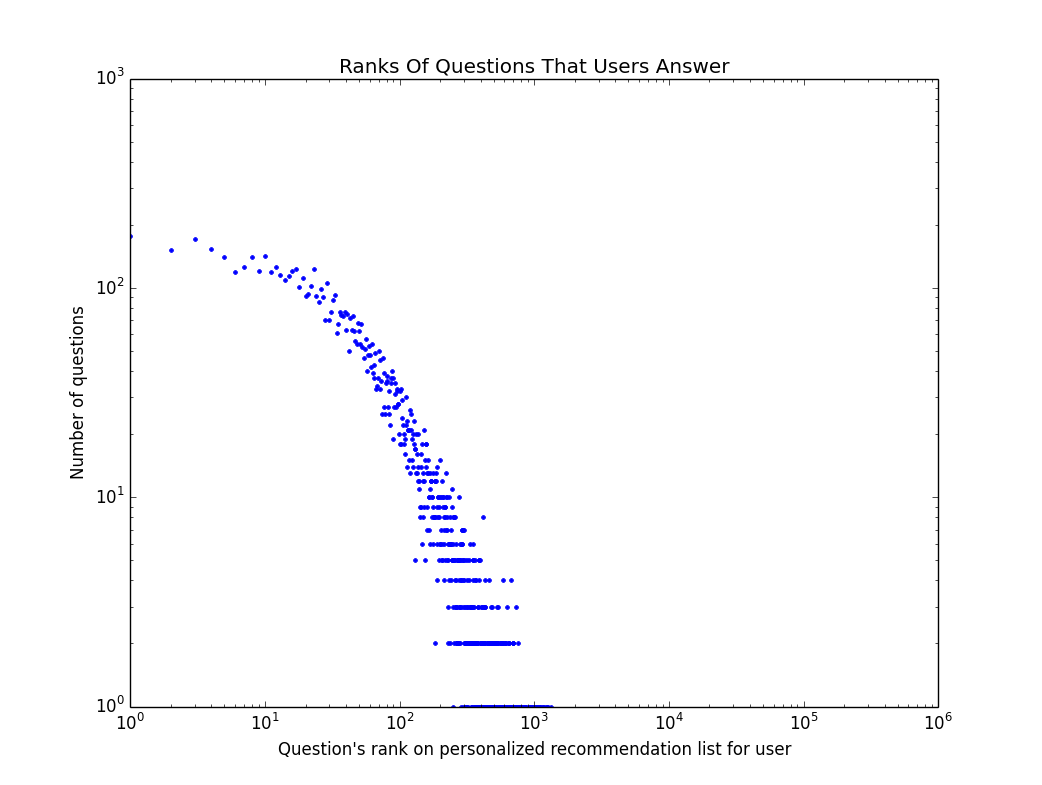
\includegraphics[width=\columnwidth]{RanksOfQuestions}
\caption{Ranks on the recommendation list that questions that the users answered would have appeared, if using the topic-relevance score alone. Plotted on log-log scales. The high concentration on the lower-ranks indicates that the tag-based topic-relevance model works well.}
\label{fig:ranks-of-questions}
\end{figure*}

If we were to take the 100 most topically relevant questions for a user, on average this would include 67\% of the questions that they answered. The median rank is 49 - meaning, if under this ranking scheme we showed the 49 top questions according to the topic-relevance model, they would include the question the user actually answered over half the time. % the average is 93.

\section{Question-Activity Model for Determining Likelihood of Answers at a Given Time}

Sites like SuperUser or StackOverflow also provide several signals that allow us to predict how likely a question will get an answer at a particular point in time. The history of past question answers, and how recently the question was asked, are relevant. For example, if a question has extremely high activity, and has received a response every minute ever since it was created, we might estimate that it's an easy-to-answer question that elicits many responses, so the probability of it getting answered at that particular timestep should be high. Likewise, if a question has 0 responses and hasn't seen any activity for a month, it is likely a very hard question to answer, so the probability of it getting answered at that timestep should be low.

%For the 

version, we intend to implement the features discussed in Anderson et al \cite{anderson2012} for predicting question activity levels, and classify a regression system to predict the probability of getting an answer to a question within a timeframe. These features include the nubmer of answers to the question, time for highest-scoring answer to arrive, scores of answers, and other features listed in their paper.

\begin{figure*}[ht]
\centering
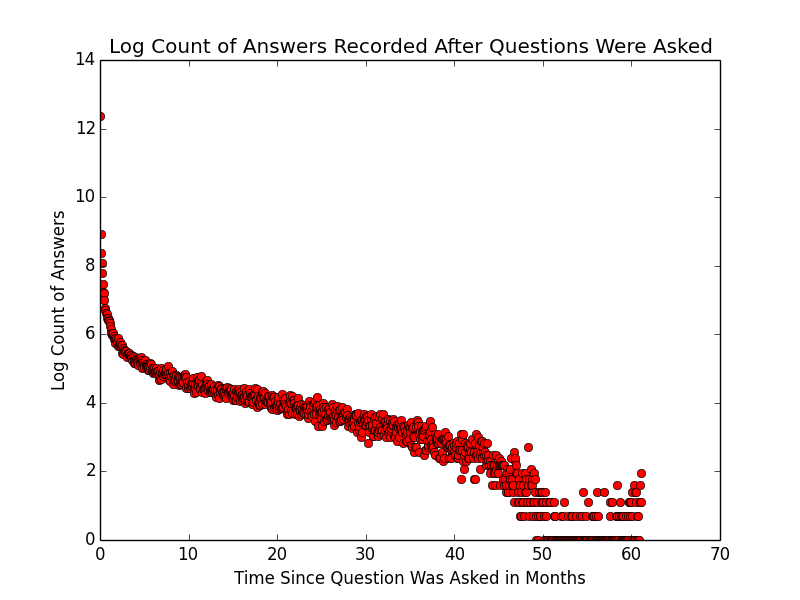
\includegraphics[width=\columnwidth]{answer-timing}
\caption{Timings at which answers come in, relative to when the question was asked. Number of answers is shown on a log scale}
\label{fig:answer-timing}
\end{figure*}

In our implementation, we train a model based on regression that considers the temporal feature of time elapsed since the question was asked to determine a future-activity score for a question. Time elapsed since the question was asked is nevertheless a useful feature; as illustrated in \ref{fig:answer-timing} the number of answers that arrive for a question is clearly a decreasing function in the amount of time since the question was asked.

The logic behind this model is based on observing that the number of new answers to a question is a decaying function in the time elapssed since the question was asked. Therefore, we bucket the number of answers to questions based on time intervals they occur on, using a log scale, because the changes in answering rate are most profound shortly after the question is asked. We smooth the histogram values with add-k smoothing to ensure that there is always a non-zero probability of someone answering a question, regardless of when it was asked. Then, when we have a new question  and time interval pair to consider, we check to see how much time has elapsed since the question was asked, and look up on our histogram what the expected number of answers arriving in this interval is. This is in turn proportional to the probability of the question getting an answer at that time (because we are interested mostly in the relative ranks of questions according to this score, rather than the probability itself, we do not need to normalize the score into a probability for our ranking purpose).

\section{Community Detection}

\begin{figure*}[ht]
\centering
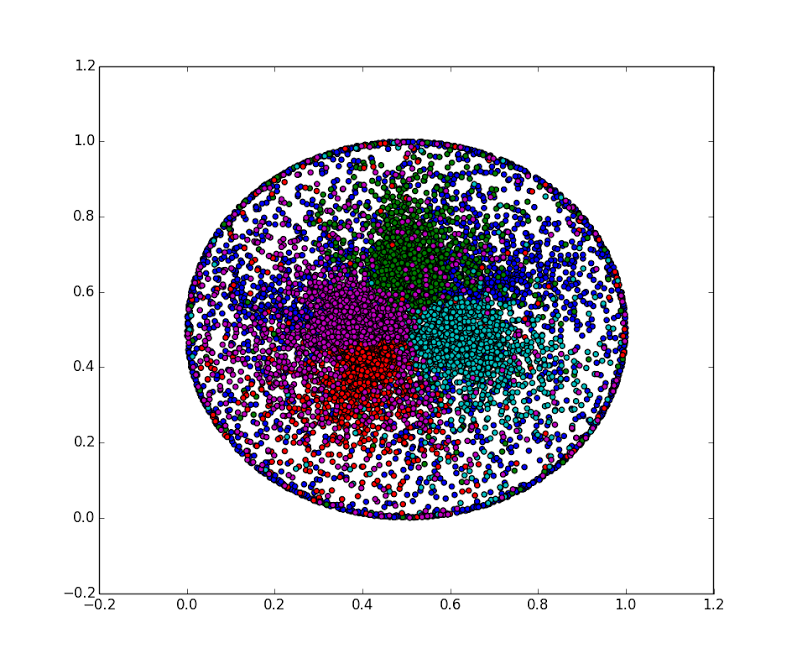
\includegraphics[width=\columnwidth]{community-detection}
\caption{Communities that are present in StackOverflow}
\label{fig:community-detection}
\end{figure*}

A limitation with our user-to-question matching based on topic similarity of tags is that for users who have only answered a few questions, the user's set of tags will only represent a small subset of their actual interests. Indeed, we found that if we consider users which have only answered a single question so far and we are attempting to predict the second question they answer, in 79.4\% of cases the second questions' tags do not overlap at all with the tags of the first question. To solve this issue, we attempt to match the user to a community, and incorporate the representative tags for the community when generating recommendations for the user.

In order to perfom community detection with users, we need a metric of user similarity. To compute similarity between a pair of users, we use the same tag-based approach as we described for user to question similarity. Namely, we take the set of tags for the pairs fo users, and perform a L2-normalized dot-product between them, with each tag weighted according to (number of questions user has answered with the tag) / (overall frequency of the tag), resulting in a user similarity metric between 0 and 1.

We then place our users on a graph, and use the user-similarity metric above to create weighted edges between them. Then we run the Louvain community detection algorithm \cite{louvian}, as implemented in the python-louvian module \cite{python-louvian}, to detect communities. We found the following major communities within the SuperUser dataset, illustrated in Figure \ref{fig:community-detection}:

The largest community appears to be Windows operating-system-centric topics. The tag set, as indicated in Figure \ref{fig:windows-tags}, shows that tags in this set are related to Windows versions (XP, Vista) and operating-system topics (networking).

\begin{figure*}
\centering

\includegraphics[width=\columnwidth]{partition0}
\caption{The tag cloud for the largest SuperUser community indicates that it focuses on Windows-centric topics. Size of tags are proportional to number of questions tagged as such.}
\label{fig:windows-tags}
\end{figure*}

\begin{figure*}
\centering
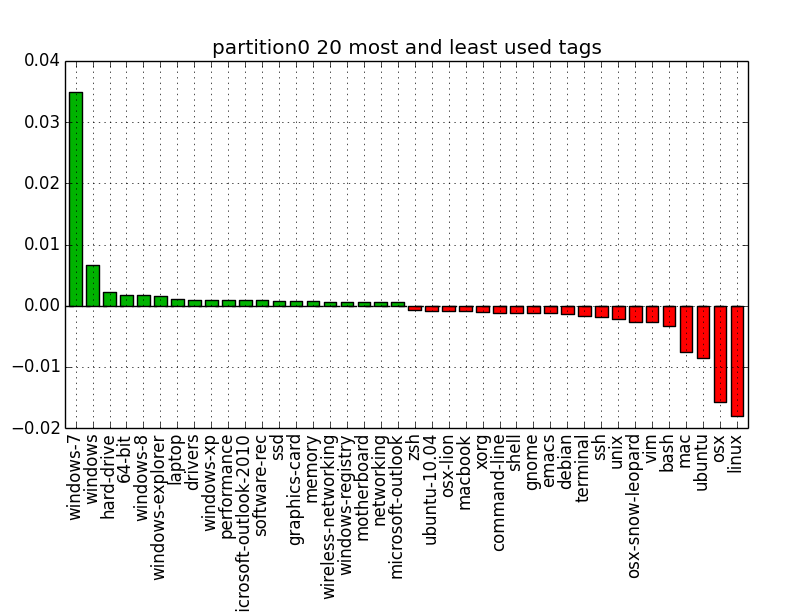
\includegraphics[width=\columnwidth]{partition0-tags}
\caption{Relative frequency of tags used by the windows (mainstream) community, consisting of mainly Windows 7 and 8 users. Zero corresponds to same frequency as an average user on SuperUser, positive values correspond to higher usage, lower values correspond to less usage.}
\label{fig:windows-tags0}
\end{figure*}

\begin{figure*}
\centering
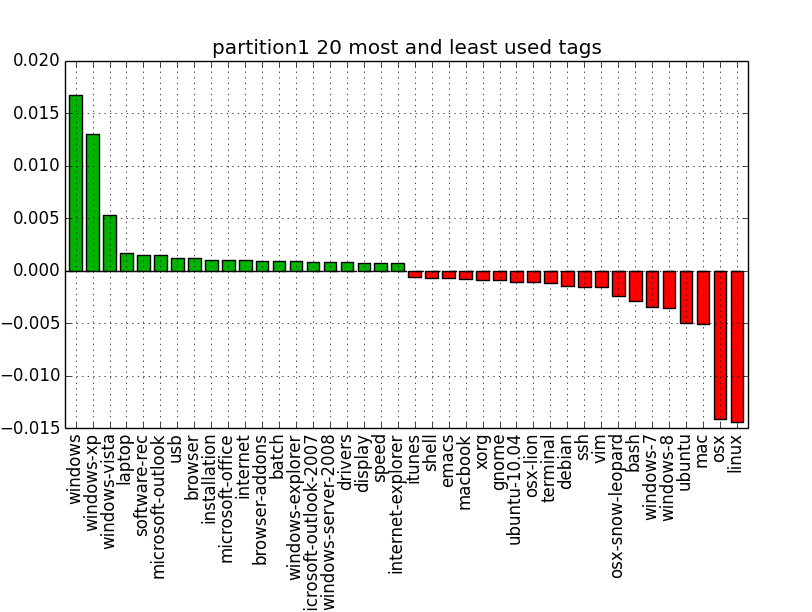
\includegraphics[width=\columnwidth]{partition1-tags}
\caption{Relative frequency of tags used by the windows (legacy) community. Observe the prevalence of Windows XP and Windows Vista-related terms compared to the mainstream Windows community.}
\label{fig:windows-tags1}
\end{figure*}


The next largest community appears to be Linux-centric topics. The tag set, as indicated in Figure \ref{fig:linux-tags}, shows names of several Linux distributions (Ubuntu, CentOS, Debian, Mint, Arch, etc) and software (emacs, bash, terminal, etc).

\begin{figure*}
\centering

\includegraphics[width=\columnwidth]{partition0}
\caption{The tag cloud for the second largest SuperUser community indicates that it focuses on Linux-centric topics. Size of tags are proportional to number of questions tagged as such.}
\label{fig:linux-tags}
\end{figure*}

\begin{figure*}
\centering
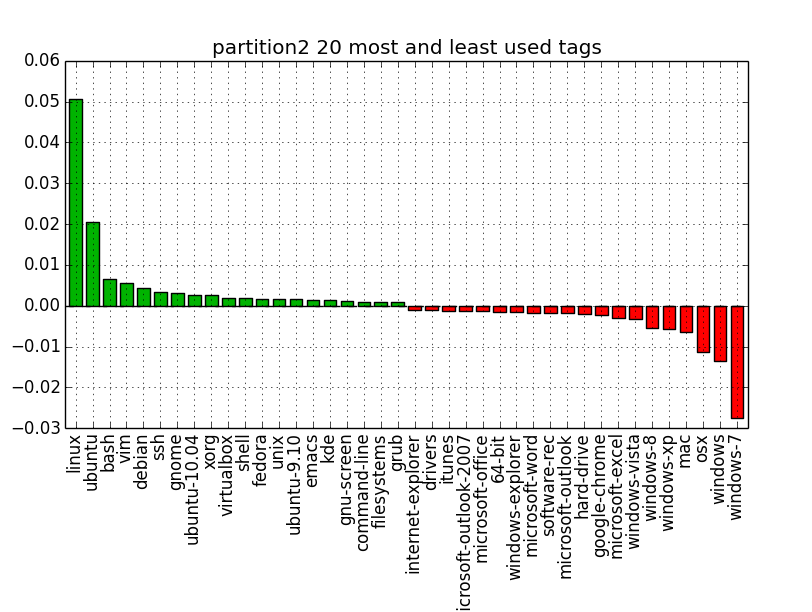
\includegraphics[width=\columnwidth]{partition2-tags}
\caption{Relative frequency of tags used by the linux community.}
\label{fig:linux-tags1}
\end{figure*}


\begin{figure*}
\centering
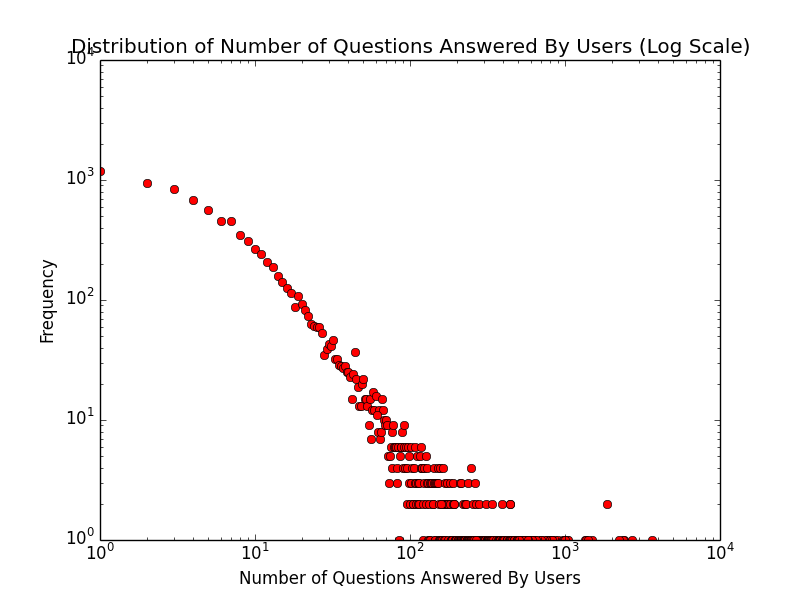
\includegraphics[width=\columnwidth]{users-to-questions-answered}
\caption{The distribution of users' question-answering activity follows a power law, as indicated in this log-log axis plot.}
\label{fig:users-to-questions-answered}
\end{figure*}

The other large communities include one on Mac OS X-centric topics, and one on Microsoft Office-centric topics.

\begin{figure*}
\centering
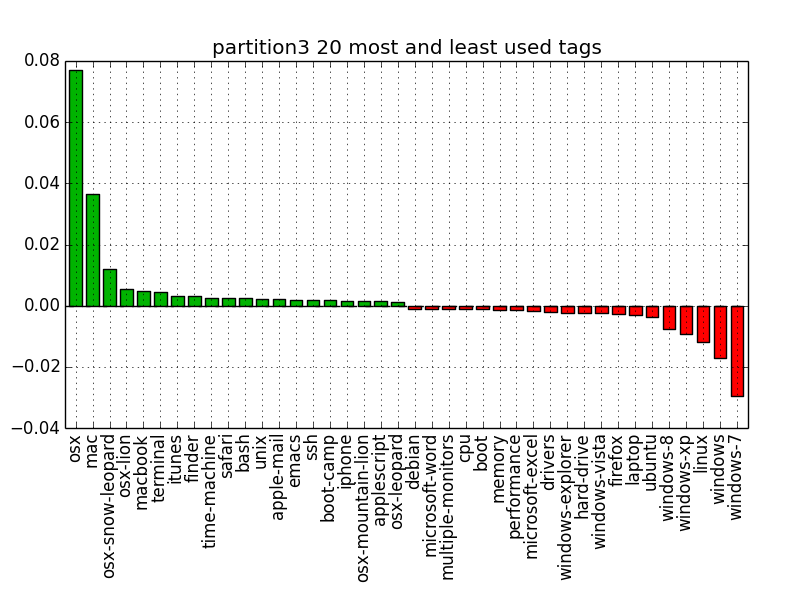
\includegraphics[width=\columnwidth]{partition3-tags}
\caption{Relative frequency of tags used by the mac community.}
\label{fig:mac-tags}
\end{figure*}

\begin{figure*}
\centering
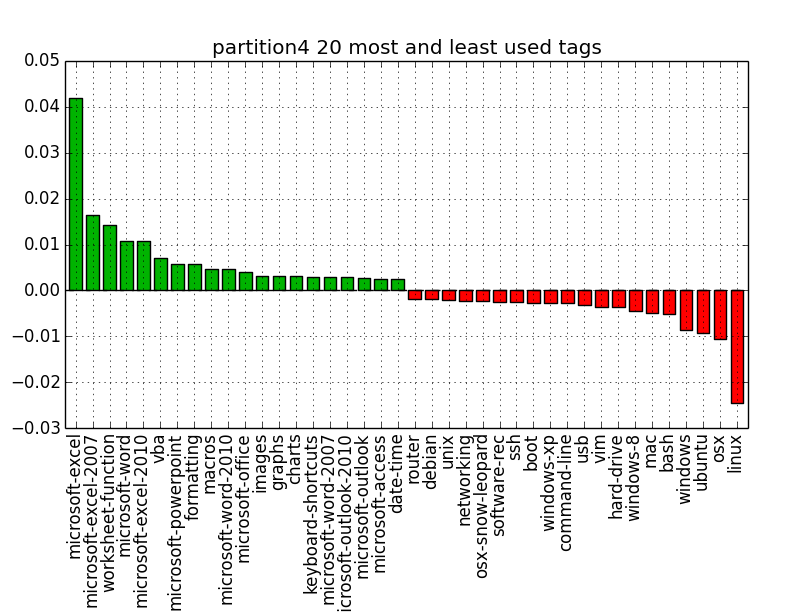
\includegraphics[width=\columnwidth]{partition4-tags}
\caption{Relative frequency of tags used by the Microsoft Office community.}
\label{fig:msoffice-tags}
\end{figure*}

After we have detected the communities in the network, we then determine a set of weighted tags for the community, by averaging over the tags for members of that community. Then, for each user, we interpolate the community-level tags, for the community they belong to, with their personal tags. This is particularly useful for generating recommendations for users with limited activity on the sites, where their interests are much broader than just the tags that they have previously answered questions for. As we can see in Figure \ref{fig:users-to-questions-answered}, the distribution of users' question-answering activity follows a power law, hence for the bulk of users we will have only a few questions answered, and hence only a few tags to work with, hence the interpolation with community-level tags is necessary for these users.

\section{Notes on the Dataset}

Before we dive into the evaluation process and results for our algorithm, we will present an overview of properties of the dataset we used.

We have originally aimed to do our evaluation on the full StackOverflow dataset from StackExchange \cite{stackexchange}, but due to our inability to get appropriate computational resources for processing it, here we are actually using the SuperUser dataset instead, which is also from StackExchange. SuperUser is a sister site of StackOverflow with the same data format, and we are using it for now because we were encountering disk space and out-of-memory issues when using StackOverflow due to the scale of the data. We also restricted to only the 10,000 users with the highest reputation - again, due to disk and memory shortage issues, we could not evaluate on all users, and we believed that the most active users are the most interesting to analyze, because we cannot personalize recommendations as effectively for users with little history of answering questions on the site.

\begin{itemize}
\item Total number of users in dataset: 181,621
\item Total number of answers: 314087
\item Total number of answers by top 10,000 users (sorted by reputation): 218210
\item Total number of questions: 185,338
\item Total number of answered questions: 159,950
\item Number of unique tags in dataset: 5,070
\item Number of elements in P(Q,U) matrix, ie num of question, user predictions: 439,903,995
\item 180 thousand questions
\item 160 thousand if we remove the ones which were unanswered (there were 20 thousand of those)
\end{itemize}


\section{Evaluation of Combined Topical-Relevance and Question-Activity Model}

Our evaluation looks at the distribution of what rank the actual question that the user answered occurs in the list of questions recommended by our recommendation system.

Let us define a \emph{question-answering event} as a tuple (time, user, question) which states that at a particular time, a user answered a particular question. We view the events in the StackOverflow dataset in chronological order, and for each event, generate a list of question recommendations using the user and time component (by computing $P(Q|T,U)$ for all questions and sorting by it). We then see how well the recommender system worked by seeing where on this list the actual question answered is ranked - that is, if we were to show a recommendation list for that user at that time, how far down they'd need to scroll to find the question they actually ended up answering. For a good recommender system, we would hope that it would have a low rank for most questions.

To clarify, pseudocode for computing the ranks used in the evaluation process is presented below, where $P(question|user, time)$ is the score output by the model to indicate how likely it is that a question is answered by a given user at a given time.

\begin{verbatim}
ranks = []
for time,user,actual_question_answered in question_answering_events:
  question_scores = []
  for question in all_questions:
    score = P(question|user, time)
    question_scores.append((score, question))
  question_scores = reverse(sorted(question_scores))
  for rank,score_and_question in enumerate(question_scores)
    score,question = score_and_question
    if actual_question_answered == question:
      ranks.append(rank)
      break
\end{verbatim}

We ran our evaluations in 3 conditions, to generate histograms of ranks:

\begin{itemize}
\item Topic-relevance model in isolation
\item Question-activity model in isolation
\item Combined prediction model
\end{itemize}

We found that the median rank score for running the combined prediction model (median score 29, histogram shown in Figure \ref{fig:results-0}) was smaller than for the topic-relevance model in isolation (median score 19219, histogram shown in Figure \ref{fig:results-1}), or for the question-activity model in isolation (median score 118, histogram shown in Figure \ref{fig:results-2}). The fact that combined prediction model's median rank score was 29 means that at least 50\% of the time, the question the user actually ends up answering at that time will be among the top 29 questions suggested by our recommendation model.

\begin{figure*}
\centering
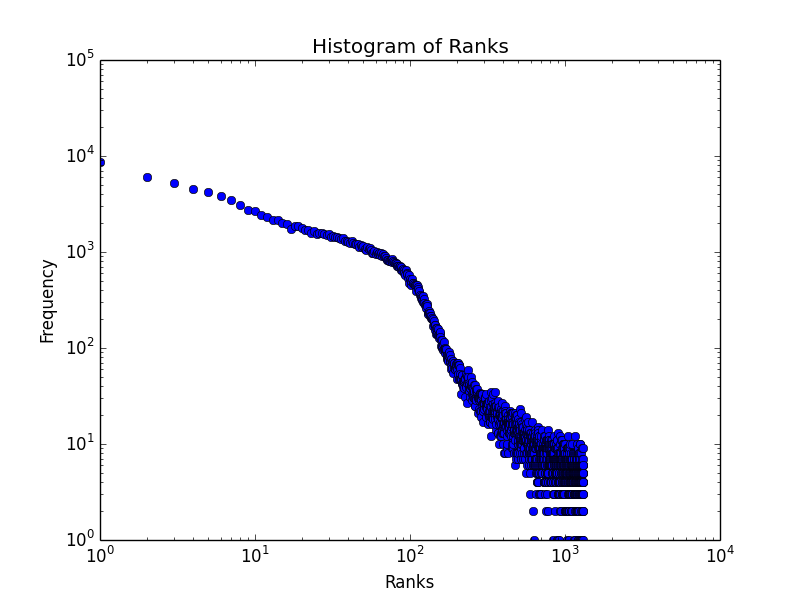
\includegraphics[width=\columnwidth]{results-0}
\caption{Histogram of ranks for recommendations, for the combined model.}
\label{fig:results-0}
\end{figure*}

\begin{figure*}
\centering
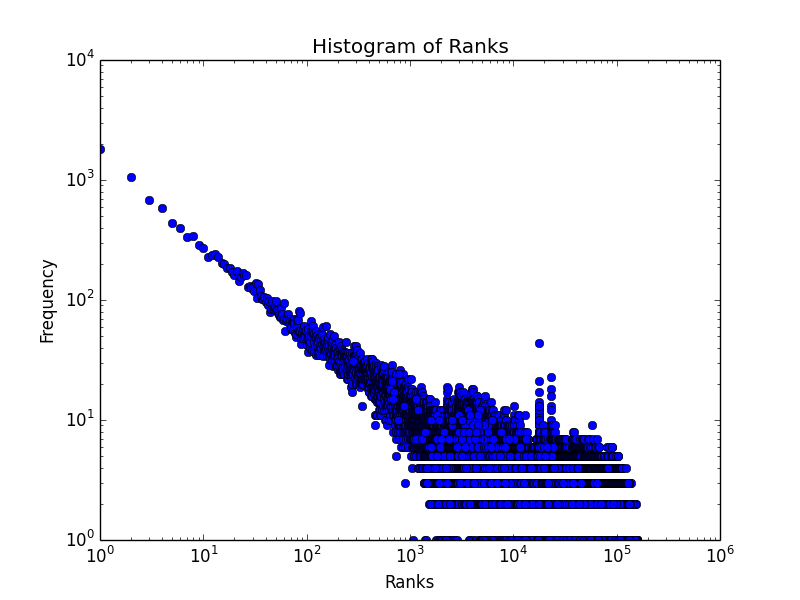
\includegraphics[width=\columnwidth]{results-1}
\caption{Histogram of ranks for recommendations, for the topic-relevance model in isolation.}
\label{fig:results-1}
\end{figure*}

\begin{figure*}
\centering
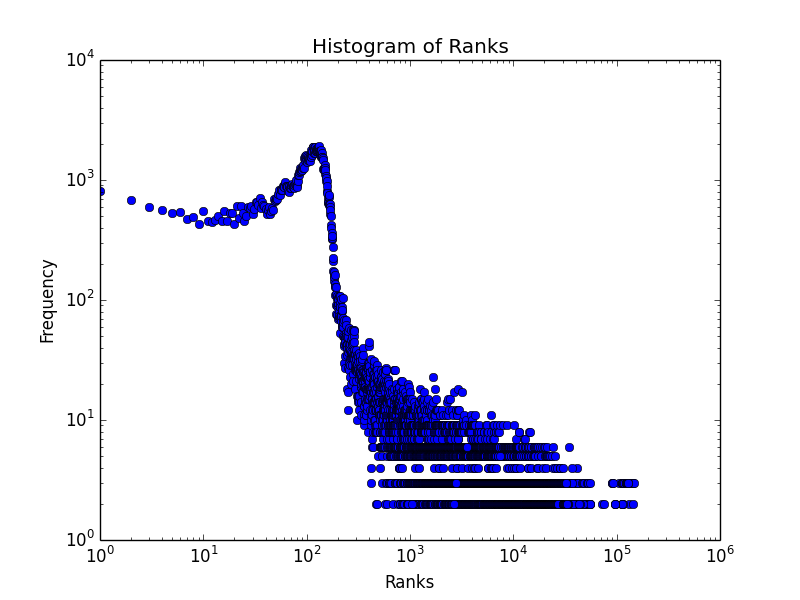
\includegraphics[width=\columnwidth]{results-2}
\caption{Histogram of ranks for recommendations, for the question-activity model in isolation.}
\label{fig:results-2}
\end{figure*}

We also seperately evaluate the effectiveness of using tags from the community to supplement the tags for users with limited history on the site, by looking at users who in total had answered only 2 questions. We found that the second question and the first question did not overlap in tags at all on 79.4\% of users. Hence it is useful to interpolate the tags from the community when generating questions for these users.

%We aim to generate histogtrams of running these evaluations for our combined prediction model, and the isolated topic-relevance and question-activity models, so we can see how much improvement combinding the two scores give us. We were unable to include them in this report due to computational resource limitations preventing us from finishing running the full evaluation before the deadline (we estimate it should finish running within 3 days). However sampling across a subset of the question-answering events suggests that the distribution of ranks of the questions actually answered within the recommendation lists are generally below 100, so the top 100 recommendations under our combined model will usually include the question actually answered.

\section{Discussion and Conclusion}

The original approach that we used for matching users to questions, of relying primarily on the questions the user has previously answered, has the limitation that the new question might not overlap with the previously answered questions' tags, particularly if the user has only answered a single or just a few questions so far. This is what our approach of detecting communities of users with related interests, matching the user to a community, and adding the community-level tags to the recommendation process aimed to solve. Tag clustering based on synonyms (as we might determine via WordNet \cite{wordnet} or a similar corpus) or co-occurrences of tags within questions might also have accomplished a similar goal of recommendation topic diversification. However, we think basing it on user community detection is preferable, because there may exist certain pairs of topics that are not directly related, but which the same set of user participate in, which our approach would help in. %For example, looking at the set of tags in the largest community, as shown in Figure \ref{fig:windows-tags}, we detected, in addition to topics related to Microsoft's operating systems, there are also 

%We generated histograms of running these evaluations for our combined prediction model, and the isolated topic-relevance and question-activity models, so we can see how much improvement combinding the two scores give us. They are shown below.

%PUT THE RANK HISTOGRAMS FOR THE 3 MODELS HERE

%\section{Remaining Work to be Done}

%For our milestone report, we have implemented a basic version of both the topic-relevance as well as the question-activity models. We have also implemented the evaluation system which uses these combined signals to generate recommendations and see how they match with what questions the users actually answered. Due to the large computation involved in our evaluation - the running time is O(answers * questions) - we were unable to do the full computation, however preliminary analysis on small subsets suggests that the median rank of questions the users actually answered on the recommendations list is less than 100, and both the topic-relevance model as well as the appear to function well individually, so our approach appears to be working.

%Work that remains to be done includes adding features to make both of these individual models more robus - for example, considering unigrams/bigrams present in the title text for our topic-relevance model, and considering the number and timing of existing answers which have arrived for questions in our activity-relevance model.

%An issue we have been running into consistently is computational resources - we were unable to run our evaluation on the full StackOverflow dataset due to constantly running out of RAM, and/or computations requiring days to complete. We aim to start using high-performance computing resources rather than our personal machines to allow us to actually work with a larger portion of the full dataset for our final evaluation.

\bibliography{midpoint}

\end{document}